\documentclass[10pt,letterpaper,xcolor=dvipsnames]{beamer}

%\usepackage[colorlinks=true,linkcolor=blue]{hyperref}
\usepackage{amssymb,mathabx}
\usepackage{linguex}
\usepackage{verbatim,enumerate,multirow}
\usepackage{xcolor}
%\usepackage{floatflt}

\usepackage{pgfpages} % to put several slides on one page
%\pgfpagesuselayout{4 on 1}[letterpaper, landscape, border shrink=5mm]

\mode<article>{}

%Template themes
\usetheme{boxes}
%\useoutertheme{miniframes}
\useoutertheme{shadow}

%Templates
\setbeamertemplate{blocks}[rounded][shadow=true]
\setbeamertemplate{navigation symbols}[vertical]
\setbeamertemplate{section in head/foot shaded}[default][20]
\setbeamertemplate{title}

\setbeamertemplate{headline}
{
	\begin{beamercolorbox}[ht=3ex,dp=1ex]{erikcolor1}
		\insertshorttitle
		%\insertsectionnavigationhorizontal{\textwidth}{}{}
		%\usebeamerfont{title in head/foot}
	\end{beamercolorbox}
	\begin{beamercolorbox}[ht=3ex,dp=2ex]{erikcolor2}
	  \insertsectionnavigationhorizontal{\textwidth}{}{}
		%\insertsubsectionnavigationhorizontal{\textwidth}{}{}
		%\insertsubsection
	\end{beamercolorbox}
}
\setbeamertemplate{footline}
{
	\begin{beamercolorbox}[ht=3ex,dp=1ex]{erikcolor1}
		\insertshortinstitute[width=.33\textwidth,center] %$\triangleright$
		\insertshortsubtitle[width=.33\textwidth,center] %$\triangleright$
		\insertshortdate[width=.20\textwidth,center] %$\triangleright$
		\hfill\insertframenumber\,/\,\inserttotalframenumber\;\;\;
	\end{beamercolorbox}
}

%Font themes
\usefonttheme{structuresmallcapsserif}
%\usefonttheme[onlysmall]{structurebold}
\usefonttheme{serif}

%Color themes
%\usecolortheme{beetle}
%\usecolortheme{rose}

%Head and foot lines colors
\setbeamercolor{erikcolor1}{fg=white,bg=blue!70!green}
\setbeamercolor{erikcolor2}{fg=white,bg=blue!60!green!10!white}

%Titles color
\setbeamercolor{frametitle}{fg=black,bg=green!30!blue!30!white}
\setbeamercolor{title}{fg=black,bg=green!30!blue!30!white}

%Block color
\setbeamercolor{block title}{fg=white,bg=blue!70!green}
\setbeamercolor{block body}{fg=black,bg=green!30!blue!30!white}

%Background color
\setbeamercolor{background canvas}{bg=}

%Covered items color
\setbeamercovered{transparent}

\AtBeginSection[]
{
   \begin{frame}<beamer>
       \frametitle{Lecture plan}
       \tableofcontents[currentsection,currentsubsection]
   \end{frame}
}



\title{Informal fallacies}
\subtitle{Relevance and weak induction}
\author[Hoversten]{Erik Hoversten}
\institute[lrp-f14]{Logic, reason, and persuasion: fall 2014 \\ Rutgers University}
\date[09/22/2014]{September 22, 2014}

\begin{document}

\begin{frame}
\titlepage
\end{frame}

\section{Fallacies in general}

\begin{frame}
\frametitle{Non sequitur}
\framesubtitle{It does not follow...}

\begin{block}{Fallacies in general...}
  \begin{itemize}
    \item are problems with the \textit{reasoning} involved in an argument.
    \item they may work by creating an \textit{illusion} that the conclusion is well supported when it is not.
    \item \textbf{non sequitur}: the conclusion is not \textit{supported} by the premises.
  \end{itemize}
\end{block}

\begin{block}<2->{Formal fallacies...}
  \begin{itemize}
    \item involve problems that can be traced exclusively to the form (or structure) of the argument.
    \item they are specific, common ways in which deductive arguments can go wrong.
    \item since they involve the reasoning of deductive arguments, they are problems with the argument's \textit{validity}.
  \end{itemize}
\end{block}

\end{frame}

\begin{frame}
\frametitle{Non sequitur}
\framesubtitle{It does not follow...}

\begin{block}{Informal fallacies...}
  \begin{itemize}
    \item are united by the fact that to determine the problem with the reasoning, we must know something about the \textit{content} of the premises used in the argument.
    \item they can be found in either deductive or inductive arguments.
    \item we'll make use of our distinctions between kinds of reasons and kinds of meaning to detect them.
  \end{itemize}
\end{block}
   
\begin{block}<2->{Kinds of informal fallacy}
  \begin{itemize}
    \item Fallacies of relevance
    \item Fallacies of weak induction
    \item Fallacies of presumption
    \item Fallacies in ordinary language
  \end{itemize}
\end{block}

\end{frame}

\section{Fallacies of relevance}

\begin{frame}
\frametitle{Fallacies of relevance}

When one commits a fallacy of this type, they present an argument that isn't relevant to the original dispute.

\begin{block}{Types}
  \begin{itemize}
    \item Appeal to force
    \item Appeal to pity
    \item Appeal to the people
    \item Against the person
    \item Straw man
    \item Red herring
  \end{itemize}
\end{block}

\end{frame}

\begin{frame}
  \frametitle{Appeal to force}
  
  \begin{block}{Argumentum ad baculum}
    \begin{itemize}
      \item The author uses a threat to try to get the reader to accept the conclusion.
      \item The threat may be convincing, but it isn't relevant to the truth of the conclusion.
      \item Compare: epistemic vs. pragmatic reason for belief.
    \end{itemize}
  \end{block}
  
  
  \begin{center}
    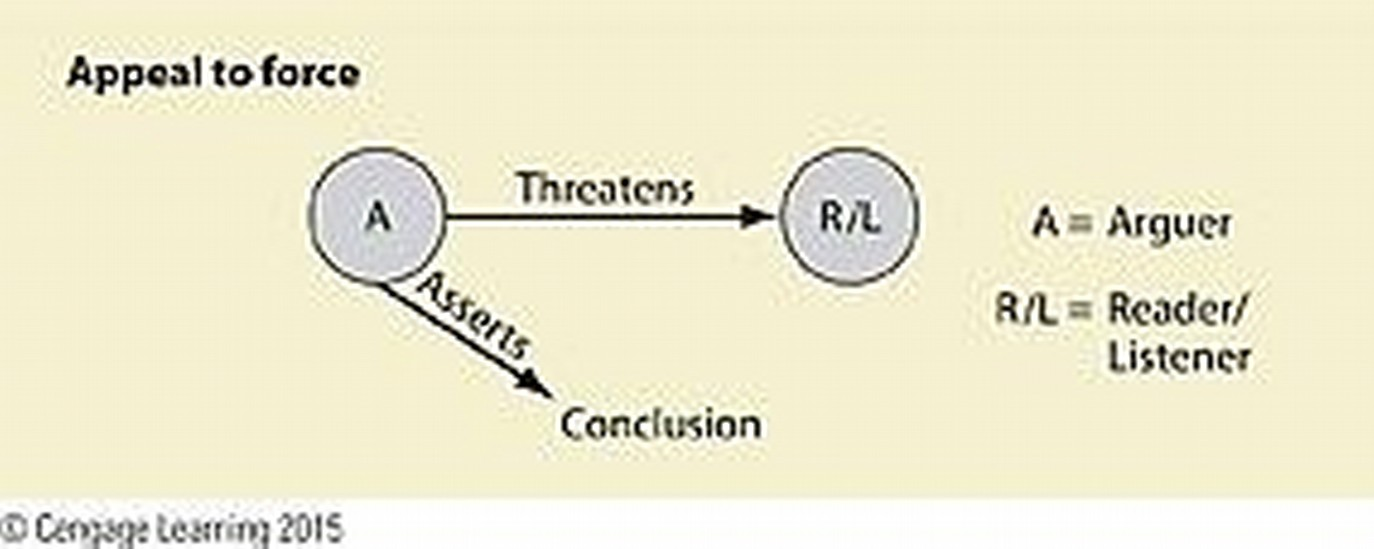
\includegraphics[width=.5\textwidth]{appeal-force.jpg}
  \end{center}
  
\end{frame}

\begin{frame}
  \frametitle{Appeal to force}
  \framesubtitle{Examples}
  
  \begin{block}{Threat of physical harm}
    ``Sure, you can root for the Jets in this game.  I'll break every bone in your body, but yeah, maybe the Jets are better.''
  \end{block}
  
  \begin{block}<2->{Threat of psychological harm}
    ``If you come out with the report about our company, I'll leak the information about your love affair last year.  It will be all over the news.  You'll never live it down.''
  \end{block}
  
\end{frame}

\begin{frame}
  \frametitle{Appeal to pity}
  
  \begin{block}{Argumentum ad misericordiam}
    \begin{itemize}
      \item The arguer attempts to support a conclusion by evoking pity from the reader.
      \item The arguer wants the reader to feel for him/her, and come to support him/her.
      \item But this emotional support is not relevant to the truth of the conclusion.
    \end{itemize}
  \end{block}
  
  \begin{center}
    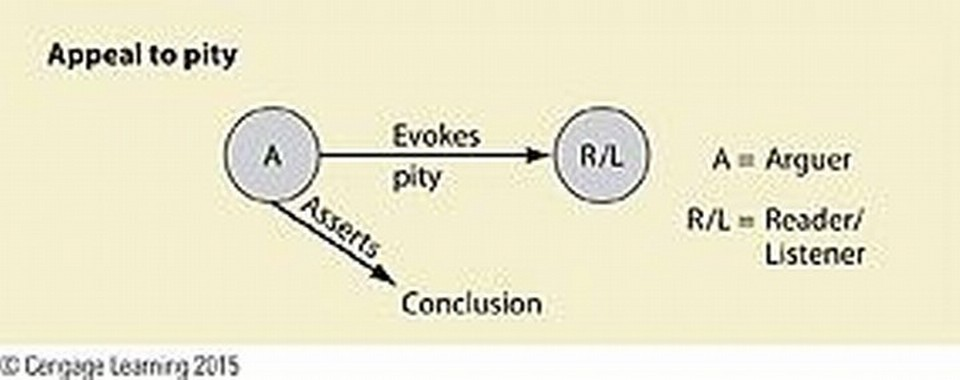
\includegraphics[width=.5\textwidth]{appeal-pity.jpg}
  \end{center}
  
\end{frame}

\begin{frame}
  \frametitle{Appeal to pity}
  \framesubtitle{Examples}
  
  \begin{block}{Defense attorney}
  ``Members of the jury, surely you will not find defendant Carlos guilty of burglary.  Carlos is a visitor from our neighbor to the south, where he has eight young brothers and sisters.  Those poor kids and their impoverished mother live a desperate hand-to-mouth existence.  Carlos was hoping only to send a few more dollars home to ease their suffering.  In the name of humanity, you must vote to acquit this caring brother.''
  \end{block}
  
  \uncover<2->{Carlos' family situation may be a good reason to have \textbf{leniency} on him during sentencing.  But it is not relevant to the issue of whether he committed the crime or not.}
  
\end{frame}

\begin{frame}
  \frametitle{Appeal to the people}
  
  \begin{block}{Argumentum ad populum}
    \begin{itemize}
      \item In addition to pity, the arguer can attempt to evoke other emotions in the reader:
      \item Effective orators will often use the psychological intensity of group energy to incite belief and action in people.
      \item Compare: cognitive vs. emotive meaning.
    \end{itemize}
  \end{block}
  
  \begin{block}<2->{Mob mentality}
    \begin{itemize}
      \item Fear: ``Our way of life is under attack!''
      \item Belonging: ``Tattoos are all the rage.  I can't believe you don't have one!'' 
      \item Vanity: ``Matt Damon eats healthy and recycles,  I can't believe you still throw away water bottles!''
      \item Tradition: ``We've always done it this way.  We can't change now!''
    \end{itemize}
  \end{block}
  
\end{frame}

\begin{frame}
  \frametitle{Against the person}
  
  \begin{block}{Argumentum ad hominem}
    \begin{itemize}
      \item The arguer \textit{shifts} their attack from the person's conclusion onto the person herself.
      \item The arguer tres to defame someone's character in order to make their conclusion less appealing.
    \end{itemize}
  \end{block}
  
  \begin{center}
    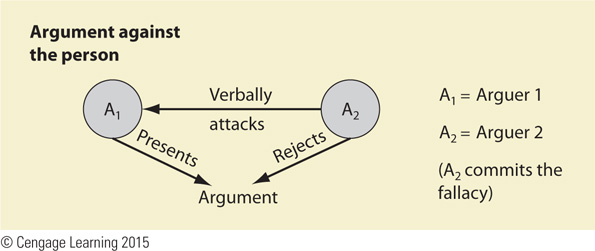
\includegraphics[width=.5\textwidth]{against-person.jpg}
  \end{center}
  
\end{frame}

\begin{frame}
  \frametitle{Ad hominem}
  \framesubtitle{Examples}
  
  \begin{block}{ad hominem abusive}
    ``Chris Christie has argued that teachers' unions are out of control.  But he's a fat loud mouth, so his arguments are worthless.''
  \end{block}
  
  \begin{block}<2->{ad hominem circumstantial}
    ``Mitt Romney is opposed to allowing abortions.  But of course he argues this way; he's a white man with a lot of money.  Abortions don't affect him, so his arguments against it are pointless.'' 
  \end{block}    

\end{frame}

\begin{frame}
  \frametitle{Ad hominem}
  \framesubtitle{Examples}
  
  \begin{block}{to quoque: ``Oh yeah? So are you!''}
    ``Al Gore argues that we need to cut back on fossil fuel use.  But he flies all over the country giving talks about it!  Obviously, his arguments are bogus.''
  \end{block}
  
  \begin{itemize}
    \item<2-> Maybe it's true that Al Gore is being \textbf{hypocritical} in this instance.  He recommends a policy for personal consumption, but doesn't follow it himself.
    \item<2-> But this doesn't mean that his policy is false.  That depends on the facts about global climate change.
  \end{itemize}
  
\end{frame}

\begin{frame}
  \frametitle{Ad hominem}
  \framesubtitle{Effective appeals to the circumstances of the arguer}
  
  Not all attacks on an arguer are fallacious.  Sometimes, the cirumstances surrounding an arguer can be relevant to whether we believe their conclusion.
  
  \begin{block}<2->{Vested interest}
    \begin{enumerate}
      \item Dick Cheney claims that we should maintain a strong military force in Iraq.
      \item But Cheney has financial ties to government contractors in Iraq.
      \item He stands to make a lot of money off of our continued presence in Iraq.
      \item So, I think we should be wary of his reasons for making his claim.
    \end{enumerate}
  \end{block}
  
  \uncover<3->{This conclusion says only that we should \textit{question} whether Cheney's claims are honestly put forward.  But, we would still have to assess his \textit{argument} directly if we want to deny his conclusion.}
  
\end{frame}

\begin{frame}
  \frametitle{Straw man}
  
  \begin{block}{Challenge a weaker argument}
    \begin{itemize}
      \item First, the arguer creates a distorted version of a person's argument.
      \item The distorted version is much weaker than the original.
      \item Then, the arguer defeats the weaker argument and claims victory over the original one.
      \item The name comes from the idea of taking down a weaker (straw) substitute for the original claim.
    \end{itemize}
  \end{block}
  
  \begin{center}
    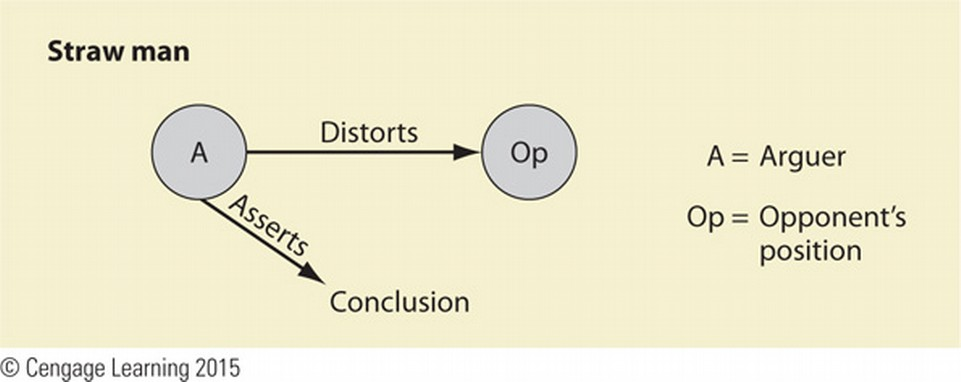
\includegraphics[width=.5\textwidth]{straw-man.jpg}
  \end{center}
  
\end{frame}

\begin{frame}
  \frametitle{Straw man}
  \framesubtitle{Examples}
  
  \begin{block}{Global warming}
    ``People are always complaining about global warming.  But look at what happened last winter.  It was one of the coldest winters I remember. We had two polar vortexes!  Obviously, the globe isn't warming that much.''
  \end{block}
  
  \begin{itemize}
    \item<2-> Here the arguer suggests that if global warming is true, then we should never see cold weather.
    \item<2-> Then he provides an example to show that is false.
    \item<2-> But, the proposed effects of global warming are very diverse.
    \item<2-> On a more \textbf{charitable} construal of global warming, the polar vortex makes perfect sense. 
  \end{itemize}  
  
\end{frame}

\begin{frame}
  \frametitle{Red herring}
  
  \begin{block}{Sneakily change the subject}
    \begin{itemize}
      \item The arguer subtly leads the discussion off topic.
      \item The hope may be that the reader may forget about the original topic and let it go.
      \item The idea comes from a technique of trying to lead dogs off the main scent by using a smelly fish as a distraction.
    \end{itemize}
  \end{block}
  
  \begin{center}
    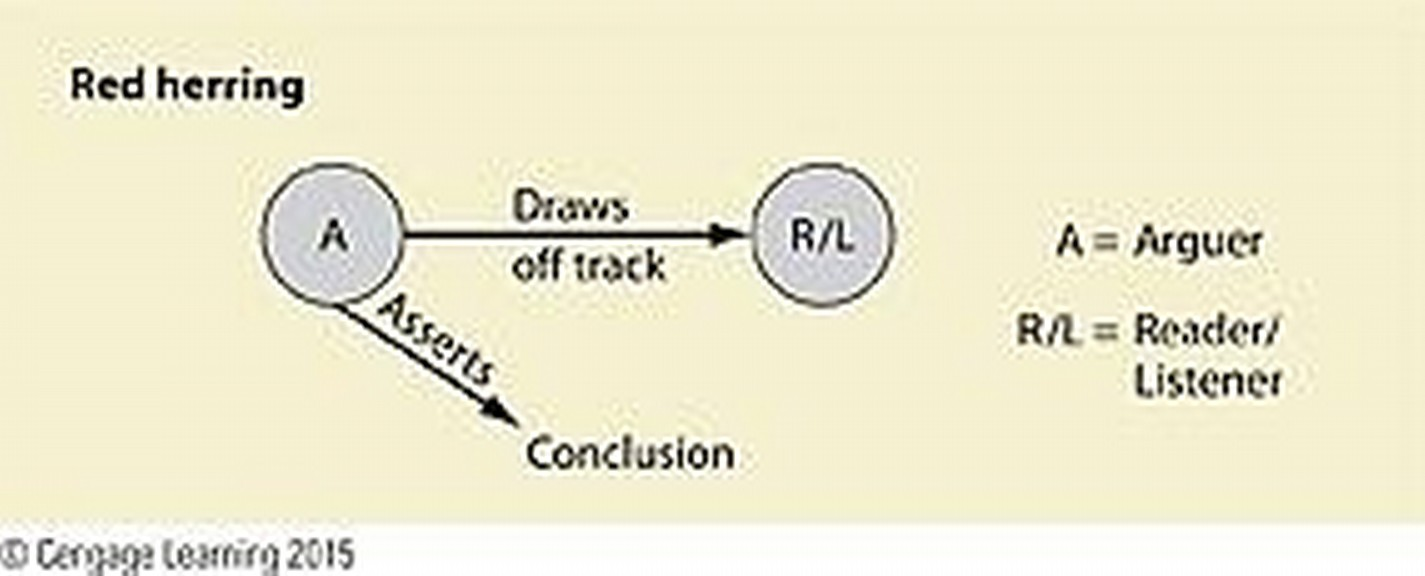
\includegraphics[width=.5\textwidth]{red-herring.jpg}
  \end{center}
  
\end{frame}

\begin{frame}
  \frametitle{Red herring}
  \framesubtitle{Examples}
  
  \begin{block}{Slight shift, plus emotional incitement}
  ``Karen argues that it's not right to post the photographs of convicted child molesters on the Internet.  Obviously, Karen supports child molestation.  But these monsters have completely ruined the lives of thousands of children.  They can't be allowed to wreak their havoc any longer.  Clearly, Karen's argument is misguided.''
  \end{block}
  
  \begin{itemize}
    \item<2-> The original topic is about posting of photographs online.
    \item<2-> But the arguer focuses on the already accepted issue that child molestation is bad.
    \item<2-> The arguer also uses emotive language to disguise the shift in topic. 
  \end{itemize}
  
\end{frame}

\section{Fallacies of weak induction}

\begin{frame}
  \frametitle{Fallacies of weak induction}
  
  This class of fallacies give us specific ways in which \textit{inductive} arguments can go wrong.  We looked at weak inductive arguments involving a bad statistical analysis.  There are a variety of other kinds of weak induction:
  
  \begin{block}{Weak induction}
    \begin{itemize}
      \item Appeal to authority
      \item Appeal to ignorance
      \item Hasty generalization
      \item False cause
      \item Slippery slope
      \item Weak analogy
    \end{itemize}
  \end{block}
  
\end{frame}

\begin{frame}
  \frametitle{Appeal to authority}
  
  \begin{block}{Argumentum ad verecundiam}
    \begin{itemize}
      \item Sometimes, we can use authorities on a subject as good evidence for a claim.
      \item But if the person we appeal to doesn't have \textit{credibility} in the subject, then the appeal lacks support.
      \item Whether the appeal is strong or not depends on the \textbf{relation} between the authority and the subject matter.
    \end{itemize}
  \end{block}
  
  \begin{center}
    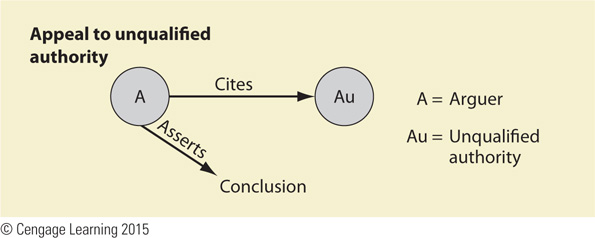
\includegraphics[width=.5\textwidth]{appeal-authority.jpg}
  \end{center}
  
\end{frame}

\begin{frame}
  \frametitle{Appeal to authority}
  \framesubtitle{Examples}
  
  \begin{block}{A bad appeal to authority}
    ``Mr. Quigley, who is a lobbyist for the oil industry, says that the government should subsidize oil exploration.  In view of Mr. Quigley's credentials, it follows that the government should certainly do this.
  \end{block}

  \begin{block}<2->{A good appeal to authority}
    ``Some members of the family don't want to let Sam go after the accident.  But the doctor's say that Sam doesn't have any brain activity, and never will again.  In light of the doctors' knowledge on the issue, I think we ought to pull the plug.''
  \end{block}

\end{frame}

\begin{frame}
  \frametitle{Appeal to ignorance}
  
  \begin{block}{Argumentum ad ignorantiam}
    \begin{itemize}
      \item Whether a claim is true or false is a different question from whether we have a \textbf{proof} of it one way or the other.
      \item When someone jumps from the claim that something hasn't been proved to the claim that it is false, they commit an appeal to \textit{ignorance}.
      \item But, if we have done a thorough investigation, and nothing has been found, this bit of ignorance can be good evidence that there is actually nothing to be found.
    \end{itemize}
  \end{block}
  
  \begin{center}
    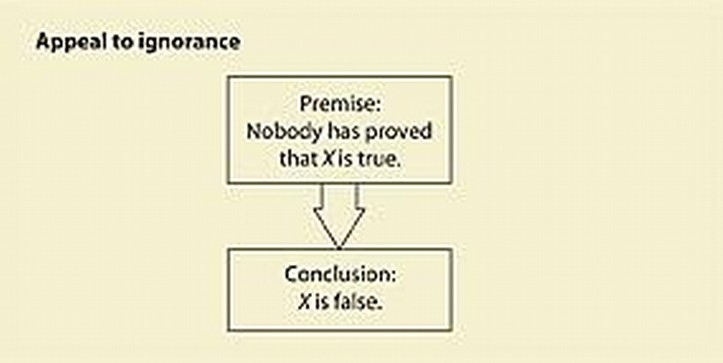
\includegraphics[width=.5\textwidth]{appeal-ignorance.jpg}
  \end{center}
  
\end{frame}

\begin{frame}
  \frametitle{Appeal to ignorance}
  \framesubtitle{examples}
  
  \begin{block}{Bad appeals to ignorance}
    \begin{itemize}
      \item ``There are lots of arguments that God exists, but I've never seen him with my own eyes.  So he doesn't exist.''
      \item ``Many people argue that God doesn't exist, but no one has proven that he doesn't.  Therefore, he does exist.''
    \end{itemize}
  \end{block}
  
  \begin{block}<2->{A good appeal to ignorance}
    ``Bill was charged with the crime.  But the police conducted a thorough investigation, and they didn't come up with a shred of evidence that Bill was at the scene.  We should conclude that Bill did not commit the crime after all.''
  \end{block}
  
\end{frame}

\begin{frame}
  \frametitle{Hasty generalization}
  
  \begin{block}{From particular to general}
    \begin{itemize}
      \item One of the main forms of inductive argument involves generalizing from \textit{examples of a phenomenon} to \textit{the whole class of phenomena}.
      \item But for the generalization to be a good one it must be based on:
      \begin{itemize}
        \item A sufficient number of example cases
        \item A representative diversity of example cases
      \end{itemize}
    \end{itemize}
  \end{block}
  
  \begin{center}
    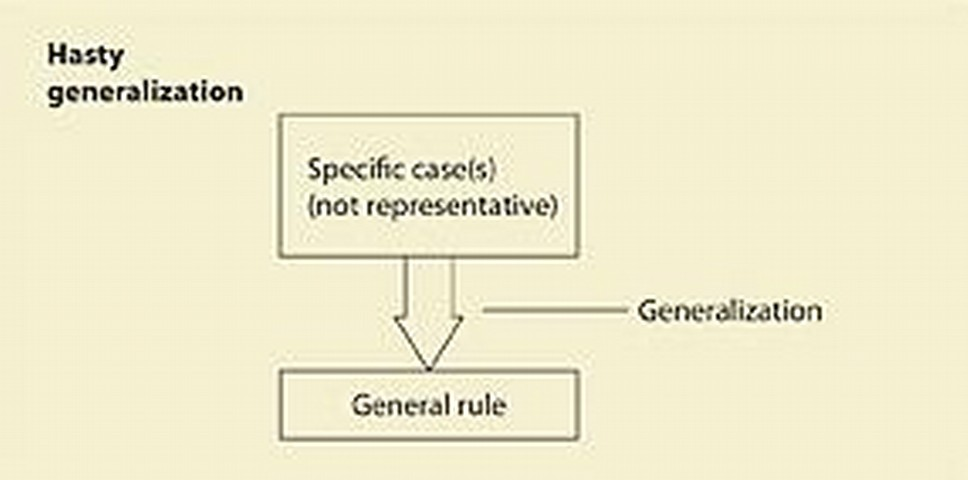
\includegraphics[width=.5\textwidth]{hasty-gen.jpg}
  \end{center}
  
\end{frame}

\begin{frame}
  \frametitle{Hasty generalization}
  \framesubtitle{Examples}
  
  \begin{block}{A bit hasty}
    ``While driving on the freeway a big truck cut me off when it changed lanes.  A few days earlier another truck tailgated me, and yet another refused to dim its lights.  The conclusion is obvious that truckers these days are as rude as they are reckless.''
  \end{block}
  
  \begin{itemize}
    \item<2-> It isn't at all clear that these two truck related incidents provide a representative example of truck driver driving courtesy.
  \end{itemize}
\end{frame}

\begin{frame}
  \frametitle{False cause}
  
  \begin{block}{That's not why it happened}
    \begin{itemize}
      \item If we know what caused a particular event, then we can be better situated to deal with events of that type in the future.
      \item But events can often be correlated, without there being a genuine causal relation betwwen them.
      \item When someone misdiagnosis the cause of an event, they commit the false cause fallacy.
    \end{itemize}
  \end{block}
  
    \begin{center}
    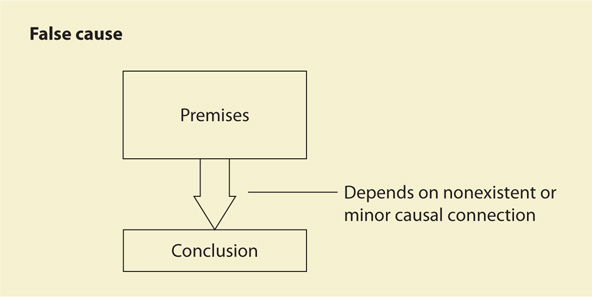
\includegraphics[width=.5\textwidth]{false-cause.jpg}
  \end{center}
  
\end{frame}

\begin{frame}
  \frametitle{False cause}
  \framesubtitle{Examples}
  
  \begin{block}{post hoc, ergo propter hoc}
    \begin{itemize}
      \item Sees that event A \textit{preceded} event B; concludes that A must have \textit{caused} B
    \end{itemize}
    
    ``Yesterday, John at a peach, and then he found \$20 on the ground.  I guess he should eat fruit more often!''
  \end{block}
  
  \begin{block}<2->{mutual cause}
    \begin{itemize}
      \item Concludes that A caused B, when A and B are each caused by event C
    \end{itemize}
    
    ``Every summer, ice cream sales skyrocket.  Crime rates also go up every summer.  So, to eliminate crime we first need to outlaw ice cream.''
  \end{block}
  
\end{frame}

\begin{frame}
  \frametitle{False cause}
  \framesubtitle{Examples}
  
  \begin{block}{Gambler's fallacy}
    \begin{itemize}
      \item Concludes that past patterns will continue, even though the events are statistically independent
    \end{itemize}
    
    ``The roulette whell has come up red the last 5 times, so I should bet heavily on red this spin!''
  \end{block}
  
\end{frame}

\begin{frame}
  \frametitle{Slippery slope}
  
  \begin{block}{If you give a mouse a cookie...}
    \begin{itemize}
      \item Events are connected, and humans are good at speculating about future chains of events.
      \item But just because a particular chain seems \textit{possible} doesn't mean that the chain is likely to arise.
      \item There may be certain events where the slide down the hill stops.
    \end{itemize}
  \end{block}
  
    \begin{center}
    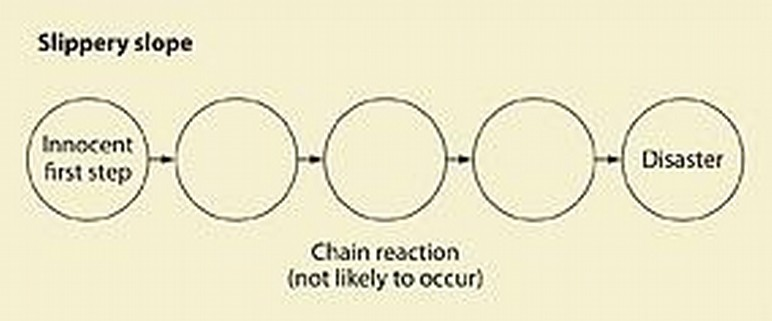
\includegraphics[width=.5\textwidth]{slippery-slope.jpg}
  \end{center}
  
\end{frame}

\begin{frame}
  \frametitle{Slippery slope}
  \framesubtitle{Examples}
  
  \begin{block}{Not so slippery}
  ``Your little Tommy wants a slingshot for his birthday, but you shouldn’t give him one.  If you do, next he’ll want a B-B gun.  Then a 22 rifle.  After that it will be a high powered rifle, and then an Uzi and an AK-47.  Soon he’ll want a bazooka and after that an antiaircraft gun.  In no time your home will become an armory.''
  \end{block}
  
    \begin{block}<2->{Maybe pretty slippery}
    ``You should avoid meth.  It's too easy to get caught up in the mess it involves.  First, you're just experimenting.  But, then you're haning out with people who don't have your best interests in mind.  Then you hav to lie to your family about what you're up too.  Eventually, you're sick, penniless, and too screwed up mentally to get out of it.  It's not worth the risk.''
  \end{block}
  
\end{frame}

\begin{frame}
  \frametitle{Weak analogy}
  
  \begin{block}{False similarity}
    \begin{itemize}
      \item If there is something about which a person is unfamiliar, a good way to describe it to them is by comparing it to something with which they are familiar.
      \item But things can be similar in one way without thereby being similar in other ways.
      \item So, analogies must show a variety of representative similiarities in order to be considered strong.
      \item Compare to hasty generalization
    \end{itemize}
  \end{block}
  
    \begin{center}
    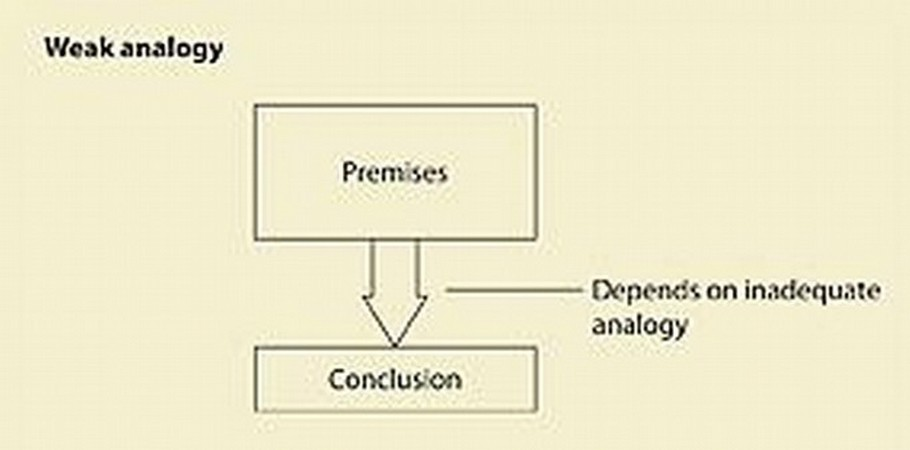
\includegraphics[width=.5\textwidth]{weak-analogy.jpg}
  \end{center}
  
\end{frame}

\begin{frame}
  \frametitle{Weak analogy}
  \framesubtitle{Examples}
  
  \begin{block}{Not much similarity}
    ``Bertha loves living in Brooklyn.  Jim and Bertha are both into food blogs, so I bet Jim would love living in Brooklyn, too.''
  \end{block}
  
  \begin{block}<2->{Non-diverse similarity}
    ``Fred and Gabe are both over six feet, lift weights, and played sports in high school, and Fred got an A in physics.  My money is on Gabe to be pretty good at physics.''
  \end{block}
  
\end{frame}

\section{Next meeting}

\begin{frame}
  \frametitle{What's coming up?}

  \begin{block}{More informal fallacies}
    \begin{itemize}
      \item Fallacies of presumption, ambiguity, and illicit transference
      \item Relevant readings: \S\S 3.4-3.5
      \item Familiarity with the various kinds of fallacy is important.  Try some of the exercises in \S3.2 and \S3.3.
      \item If you bring up one of the questions, I will tell you what answer I got for it.
    \end{itemize}
  \end{block}
  
\end{frame}

\end{document}
